\documentclass{article}
\usepackage[utf8]{inputenc}
\usepackage{graphicx}
\usepackage{subcaption}
\usepackage{amsmath}
\usepackage{tablefootnote}
\usepackage{csvsimple}
\usepackage{setspace}
\usepackage{amsthm}
\usepackage[ruled,vlined]{algorithm2e}
\usepackage{tikz}
\usepackage{blkarray}
\usetikzlibrary{arrows}
\usepackage[
  backend=biber,
  style=apa,
  citestyle=apa
]{biblatex}
\usepackage{geometry}
\geometry{
 a4paper,
 total={150mm,237mm},
 left=30mm,
 top=30mm,
 }
\newtheorem{definition}{Definition}
\newtheorem{remark}{Remark}
\newtheorem{corollary}{Corollary}
\newtheorem{theorem}{Theorem}
\def\indep{\perp \!\!\! \perp}
\def\notindep{\not\!\indep}
\renewcommand{\baselinestretch}{1.5} 
\addbibresource{references.bib}

\title{Causal Discovery of Macroeconomic State-Space Models}
\author{Emmet Hall-Hoffarth}
\date{\today}

\makeatletter
\newenvironment{chapquote}[2][2em]
  {\setlength{\@tempdima}{#1}%
   \def\chapquote@author{#2}%
   \parshape 1 \@tempdima \dimexpr\textwidth-2\@tempdima\relax%
   \itshape}
  {\par\normalfont\hfill--\ \chapquote@author\hspace*{\@tempdima}\par\bigskip}
\makeatother

\begin{document}

\maketitle

\abstract{This paper presents a set of tests and an algorithm for agnostic, data-driven selection among macroeconomic DSGE models inspired by structure learning methods for DAGs. Structure learning algorithms can be used because the log-linear state-space solution to any DSGE model is also a DAG. In particular, it is possible to define a set of conditional independence relationships which uniquely identify the ground-truth state-space model that is consistent with some underlying DGP. I then introduce an algorithm which tests feasible analogues of these criteria against the set of possible state-space models in order to converge asymptotically to the ground-truth model. In finite samples where the result may not be unique, conditional independence tests can be combined with likelihood maximisation in order to select a unique optimal model. The efficacy of this algorithm is demonstrated for simulated data, and results for real data are also provided and discussed.}

\vspace{1cm}

\begin{chapquote}{Guido Imbens, \textit{NBER, 2019}}
  "... the most important issue holding back the DAGs is the lack of convincing empirical applications. History suggests that those are what is driving the adoption of new methodologies in economics and other social sciences,  not the mathematical elegance or rhetoric."
\end{chapquote}

\section{Introduction}

In the machine-learning literature, causal discovery is generally defined as the act of inferring causal relationships from observational data \parencite{huang2020causal}. This however also exactly describes the goal of most empirical economic research and therefore in this context it is most reasonable to append to this definition that which is taken for granted in machine-learning --- that this inference is done \textit{algorithmically}. The field of (algorithmic) causal discovery has been subject to intense development in recent years, however, it is hardly new. Work along these lines started as early as the 1980's with contributions from Judea Pearl, Thomas Verma, Peter Spirtes, and others. 

While there are many approaches to causal discovery, the current paper will focus on the inference of a Directed Acyclical Graph (DAG), sometimes also referred to as a Bayesian Network. These are a type of \textit{graphical model} which can be used to illustrate, and in many cases infer causal relationships between variables. While the use of these models as a descriptive tool has been hotly debated \parencite{pearl2018book}, what is perhaps more exciting and novel for the field of economics is the fact that numerous algorithms exist which, under limited assumptions can identify a DAG, and thus a causal model, directly from observational data.

While there is a considerable potential for the application of such a tool in economics, thus far relatively little work in this vein has taken place. Indeed, \citeauthor{imbens2019potential} (\citeyear{imbens2019potential}) considers the value of DAGs for empirical economics and concludes that the reason this framework has not caught on is precisely because few useful applications have been demonstrated. This paper aims to remedy this by considering an application of DAGs to macroeconomic DSGE models. In particular, I show that a DSGE model's log-linear state-space solution can be represented as a DAG, and that the structure of that DAG, and thus that of the state-space solution, can be recovered consistently from observational data only. 

DSGE models such as the \textit{Real Business Cycle} (RBC) model first popularised by \citeauthor{kydland1982time} (\citeyear{kydland1982time}), and subsequent \textit{New Keynesian} models were formulated primarily as a response to the Lucas critique; that reduced form macroeconomic timeseries models such as VARs are unsuitable for inferring the causal effects of changes to microeconomic or structural parameters. The key feature of DSGE models is that they are based on \textit{microfoundations} --- that is, they explicitly model the optimal behaviour of representative agents in order to derive equillibrium conditions. However, these optimisation problems are still subject to assumptions about the nature of constraints faced by agents, the information available to them, and in some cases even their degree of rationality. For example, do agents form expectations in a purely forward looking fashion, or do they employ some form of indexing? In the relevant literature these assumptions are generally justified either with microeconomic evidence or comparing by the \textit{impulse response functions} generated by the model to those estimated by econometric models \parencite{christiano2018on}. 

Different assumptions about microfoundations will sometimes, but not always, imply different state-space models. In these cases, the test and algorithm presented in this paper can be seen as another tool that can be used to evaluate models. In particular, they do so in a \textit{maximally agnostic} way, with minimal assumptions that do not take any stance in particular about which relationships between variables may exist, only on the nature of these relationships, for example, linearity. What this paper does not (yet) do is present a solution to the problem of \textit{microeconmic dissonance} \parencite{levin2008macroeconometric}. In cases where the linear state-space model implied by DSGE models are equivalent, this procedure cannot determine which set of microfoundations are more reasonable.

Despite considerable promise, and theoretical guarantees of asymptotic consistency, in simulation experiments existing structure-learning algorithms for DAGs performed poorly at identifying state-space models. This is likely due to the fact that they search over the set of all possible DAGs, whereas in this context we are willing to assume that the solution is a state-space model of a specific form, and also in the macroeconomics sample sizes available are usually small relative to the number of observables. Therefore, I develop a bespoke algorithm using tools for DAG structure learning, while also integrating assumptions about the nature of the log-linear DSGE solutions, which is asymptotically consistent, and also is able to identify some solutions given realistic data sizes.

The remainder of the paper is organised as follows. Section \ref{lit_review} will cover background information on both DAGs and DSGE models. Section \ref{methodology} will introduce the proposed structure learning tests and algorithm. Section \ref{data} briefly introduces simulated and real world data which will be used for emperical validation. Section \ref{results} provides and discusses the performance of the algorithm on these data sets. Section \ref{conclusion} will conclude.  

\section{Liturature Review} \label{lit_review}

\subsection{DAGs} \label{dags}

\subsubsection{Preliminaries} \label{prelim}

\begin{figure}
  \centering
  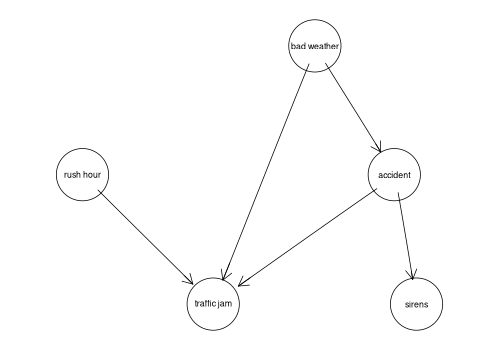
\includegraphics[width=0.75\textwidth]{images/trafficjam.png}
  \caption{A simple example of a DAG \parencite{traffic_jam}}
  \label{dag1}
\end{figure}

Formally, a DAG $G$ is a pair $(V,E)$ where $V$ is a set of \textit{nodes}, one for each of $k$ observable variables, and $E$ is a $V \times V$ set of \textit{edges} or \textit{arcs} \parencite{kalisch2007estimating}. $(x,y) \in$ $E$ indicates the presence of an directed edge from node $x$ to node $y$. As the name suggests, every edge in $E$ is directed such that if $(x,y) \in E$ then $(y,x) \not \in E$. $E$ is also assumed to not contain any cycles, that is, there is no set of edges ${(i,j)} \in E$ containing a directed path starting and ending at the same node. Figure \ref{dag1} gives a simple example of a DAG.

In general, DAGs can represent either discrete, continuous, or mixed variables, but in the current application only continuous variables will be considered. For simplicity, each arc will hereafter be assumed to define a linear relationship between continuous variables. With this assumption we can more specifically define $V$ as a $(k \times 1)$ vector and $E$ as a $k \times k$ adjacency matrix containing slope parameters, where $e_{ij} \not = 0$ indicates a directed edge from node $i$ to node $j$ and $e_{ij} = 0$ indicates the lack of an edge. The directedness assumption is analogous, and the acyclic property is equivalent to the statement that $E^n$ has zeros on its diagonal for $\forall n > 0$. The model will now also include a $k \times 1$ vector $\mathbf{\epsilon}$ containing mutually independent Gaussian shocks, one for each node.

The set of nodes from which an arc into $x$ originates are known as the \textit{parents} of $x$ ($pa_G(x)$), and the set of nodes that have an incoming arc from $x$ are known as the \textit{children} of $x$ ($ch_G(x)$). The set of all nodes from which a directed path into $x$ originates are known as the \textit{ancestors} of $x$ ($ans_G(x)$) and the set of all nodes that have an incoming path from $x$ are known as the \textit{decendents} of $x$ ($des_G(x)$). 

I will now briefly review some key results pertaining to DAGs that are utilised in this paper. For a more complete treatment see \citeauthor{pearl2009causality} (\citeyear{pearl2009causality}).

\theoremstyle{definition}
\begin{definition}{Faithfulness}
  Let $f$ represent some DGP, and $I(f)$ be the conditional independence relationships implied by $f$. A DAG $G$ with parameters $\theta \in \Theta$ is said to be \textbf{faithful} to $f$ if and only if the conditional independence relationships implied by $G$ satisfy $I(G(\theta)) = I(G(\theta^\prime)) = I(f) \text{  } \forall \text{  } \theta \not = \theta^\prime \in \Theta$.
  \parencite[p.48]{pearl2009causality}
  \label{faithfulness}
\end{definition}

Outside of the optional assumption of linearity and Gaussian errors that are made here for simplicity, \textit{faithfulness} is the only assumption necessary for the identification of a DAG for a true DGP \footnote{Note that this definition of faithfulness includes an equivalence relationship and therefore encompasses what is sometimes  referred to separately as the "causal Markov condition" which states that $I(g(\theta)) \implies I(f)$ \parencite{spirtes2016causal}}. It is the assumption that the conditional independence relationships in the DGP are \textit{stable} to perturbations of parameters. Intuitively, if we wish to use conditional independence relationships to identify a model then we must assume that the observed conditional independence relationships do not belie the underlying distribution. This assumption is only violated if some causal effects exactly cancel out, resulting in no observed correlation between casually connected variables. \citeauthor{pearl2009causality} (\citeyear{pearl2009causality}) provides the following example. Consider the following model: $z = \beta_{zx} x + \epsilon_x$, $ y = \beta_{yx} x + \beta_{yz} z + \epsilon_y$. If we impose the parameter restriction $\beta_{yx} = -\beta_{yz}\beta_{zx}$ then $x$ and $y$ are independent. However, this independence relationship is not robust to perturbations of the model parameters and is therefore not stable in the relevant sense. 

A sufficient condition for faithfulness is that the DGP parameters are jointly continuous and vary freely over the parameter space \parencite{steel2006homogeneity} for different populations, or equivalently, that the matrix of DGP parameters is of full rank. This is because under this condition, specific combinations of parameters which result in the cancellation of causal effects have has Lebesgue measure 0. If we believe that the true DGP of the macroeconomy is DSGE model, which itself is faithfully represented by a DAG, then this condition is unlikely to be met. DSGE models impose many cross-equation restrictions on parameters that effectively reduce the rank of the parameter matrix. Unfortunately this condition will not allow us to guarantee that DSGE models satisfy the faithfulness assumption. Regardless, this condition is merely sufficient, not necessary, and so it does not rule out that DSGE models can be faithfully represented by DAGs. 

In another approach to failures of faithfulness, \citeauthor{steel2006homogeneity} (\citeyear{steel2006homogeneity}) notes that such failures or near-failures (that is near-zero statistical dependence despite clear causal pathways) are likely occur when parameters are both subject to \textit{selection} and \textit{homogeneity}. In this context, selection means that parameters are entirely determined by an economic agent. The suggestion is that if the path of a policy variable $z$ is specifically designed as a function of $x$ to counteract the causal effect of $x$ on some outcome $y$, then it is reasonable to believe that little or no correlation will be observed between $x$ and $y$ despite a clear causal pathway between them. If parameters are assumed to be come from some distribution with different draws for each population, then homogeneity is the statement that there is little exogenous variation in those parameter values, that is variation outside of the variation caused by selection. If \textit{both} selection and homogeneity occur, failure or near-failure of faithfulness is likely to occur. Within the context of macroeconomics, this seems likely to be the case when considering interest rates and the actions of central banks. Assuming the interest rate is set according to a Taylor (\citeyear{taylor1993discretion}) rule, the parameters of that rule are chosen with the specific intent and cancelling the causal effect of inflationary shocks on output and minimising exogenous variation. 

Despite these concerns, I would argue that the faithfulness assumption is plausible in most macroeconomic contexts. For simulations, whether or not the assumption is violated can be read straight off the structural model. For real data, it seems unlikely that any macroeconomic variable (even the policy rate) is determined in an entirely systematic for deterministic way. In reality, monetary authorities face a number of constraints that would prevent them from completely stabilising inflation including informational constraints, political influences, and the zero lower bound. Identification of policy rate shocks has been a topic of much scrutiny \parencite{ramey2016handbook}, and this line of research has provided a significant amount of evidence for the existence of such shocks. Given that $f$ is \textit{stable} we can use conditional independence tests in the following way to evaluate whether a DAG $G$ is consistent with $f$.

\begin{definition}{D-Separation}
  A path $P$ in a DAG $G$ is said to be \textbf{d-separated} or \textbf{blocked} by a set of variables $\mathbf{z}$ if and only if: \\
  A. $P$ contains a chain $x \rightarrow m \rightarrow y$ or fork $x \leftarrow m \rightarrow y$ and $m \in \mathbf{z}$ \\
  B. $P$ contains a collider $x \rightarrow m \leftarrow y$ and $\{m \cup des(m)\} \cap \mathbf{z} = \emptyset$ \\
  A set of variables $\mathbf{z}$ is said to \textit{d-separate} $x$ and $y$ if $\mathbf{z}$ blocks every path between $x$ and $y$.
  \parencite[p.16]{pearl2009causality}
  \label{dseparation}
\end{definition}

\theoremstyle{theorem}
\begin{theorem}{D-Separation and Conditional Independence}
  If $x$ and $y$ are d-separated by $\mathbf{z}$ in DAG $G$, and $G$ is faithful to the true DGP $f$ of $x$ and $y$, then $x$ and $y$ are independent conditional on $\mathbf{z}$. 
  \parencite[p.16]{pearl2009causality}
  \label{dseptheorem}
\end{theorem}

This result is essential for defining the constraint based tests in section \ref{constrainttests}. In particular, it implies the following result that we will leverage:

\theoremstyle{corollary}
\begin{definition}{Parental Markov Condition}
  Given some DAG $G$, a node $x$ in $G$ is d-separated from and therefore independent of all its non-decendents by its parents. This is known as the \textbf{Parental Markov Condition}. 
  \parencite[p.16, p.19]{pearl2009causality}
  \label{markovcompatibility}
\end{definition}

\theoremstyle{corollary}
\begin{corollary}
  If $G$ is faithful to the DGP $f$ then $f$ admits the following factorisation:
  \begin{equation}
    f(\mathbf{w};\theta) = \prod_{i=1}^{k} f(w_i | pa_G(w_i);\theta)
  \end{equation}
\end{corollary}

\subsubsection{Estimation} \label{dag_estimation}

There are two fundamental problems to solve when estimating a DAG. The first is known as "parameter learning," and the other "structure learning." Given a DAG as in Figure \ref{dag2}, the first task is simply to estimate the parameters of the network, such as the parameter matrices $\mathbf{A}$, $\mathbf{B}$, $\mathbf{C}$, $\mathbf{D}$, and $\mathbf{E}$ in Equation \ref{ss_solution:x} - \ref{ss_solution:z}. This is usually done via maximum likelihood or with Bayesian techniques.

\begin{figure}
  \centering
  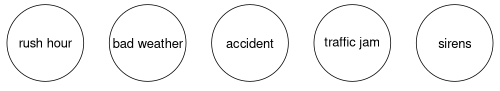
\includegraphics[width=0.75\textwidth]{images/trafficjam_unfit.png}
  \caption{A DAG before structure learning}
  \label{dag2}
\end{figure}

The second and more onerous task, as demonstrated by Figure \ref{dag2} is that if we just start with some data it is not obvious which conditional probabilities to estimate in the first place. One way to do this is for the researcher to specify explicitly which conditional probabilities should be present in the graph, and simply fit the parameters of that graph. How this can be done in the context of DSGE models is discussed in Section \ref{methodology}. In this context however, doing so achieves little. This is equivalent to specifying a system of linear regressions to be estimated, probably based on some economic model that was developed by other means, and while this is then automatically encapsulated in a convenient, easily interpreted representation of the underlying assumptions, it seems nothing particularly novel would have been achieved. 

A more exciting approach is to algorithmically learn the structure of the graph, that is to learn a causal model, directly from observed data. One "brute force" method to solving this problem is to compute the posterior likelihood of every possible network, however, this number is super-exponential in the number of variables and therefore it becomes very computationally expensive, very quickly \parencite{chickering1996learning}. As a response to this, many heuristic approximation techniques have been developed. These can be grouped into two categories: constraint-based and score-based structure learning algorithms \parencite{spirtes1991algorithm} \parencite{verma1991equivalence}. 

\begin{figure}
  \centering
  \begin{subfigure}{0.3\textwidth}
    \centering
    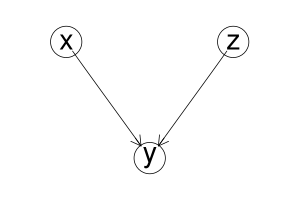
\includegraphics[width=\linewidth]{images/collider.png} 
    \small
    \begin{equation*}
      x = \epsilon_{x}
    \end{equation*}
    \begin{equation*}
      y = \beta_{yx} x + \beta_{yz} z + \epsilon_{y}
    \end{equation*}
    \begin{equation*}
      z = \epsilon_{z}
    \end{equation*}
    \caption{Collider}
    \label{collider}
  \end{subfigure}
  %
  \begin{subfigure}{0.3\textwidth}
    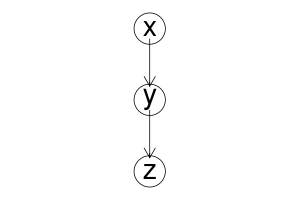
\includegraphics[width=\linewidth]{images/chain.png}
    \small
    \begin{equation*}
      x = \epsilon_{x}
    \end{equation*}
    \begin{equation*}
      y = \beta_{yx} x + \epsilon_{y}
    \end{equation*}
    \begin{equation*}
      z = \beta_{zy} y + \epsilon_{z}
    \end{equation*}
    \caption{Chain}
    \label{chain}
  \end{subfigure}
  %
  \begin{subfigure}{0.3\textwidth}
    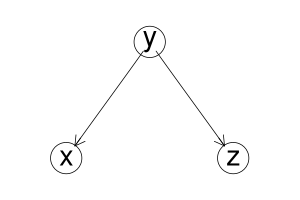
\includegraphics[width=\linewidth]{images/fork.png}
    \small
    \begin{equation*}
      x = \alpha_x + \beta_{xy} y + \epsilon_{x}
    \end{equation*}
    \begin{equation*}
      y = \epsilon_{y}
    \end{equation*}
    \begin{equation*}
      z = \beta_{zy} y + \epsilon_{z}
    \end{equation*}
    \caption{Fork}
    \label{fork}
  \end{subfigure}

  \caption{The three possible v-structures of a 3 node DAG. Error terms $\epsilon$ are all i.i.d. Gaussian shocks.}
  \label{dag5}
\end{figure}

Constraint-based algorithms rely on the fact that changing the direction of an arc changes the conditional independence relationships implied by the graph, the presence of which can be tested for in the data. To see how the DAG assumptions can be sufficient to learn a causal model in this way, consider the example in figure \ref{dag5}. Suppose we have a graph with three nodes, such that no one node is completely independent from the other two (as this would make the graph trivial, and we could in any case rule out this case with an independence test). Furthermore, the graph cannot have all three possible arcs because it would either contain a cycle, or the third arc would imply a relationship which is redundant given the other two. Then the graph must have exactly two arcs. Given this, there are exactly three possible permutations of the network, which are the three shown in figure \ref{dag5}. These are known as the the three canonical "v-structures." \parencite{pearl2014probabilistic} These structures are partially identifiable from observational data because they imply different testable hypotheses about conditional independence. While the chain and fork imply that x and z are unconditionally dependent and only independent conditional on y, the collider implies exactly the opposite; that x and z are unconditionally independent and dependent conditional on y. Given some observed data we can easily test for the presence of conditional and unconditional independence under the assumption of joint-normality using a t-test or F-test on (partial) correlations. The results of these tests can be used to rule out certain network structures which would be inconsistent with the observed data. Although for every set of three variables the network is only partially identifiable, full identification can (but will not always) be achieved when more variables are observed, by comparing overlapping triplets of variables and progressively reducing the set of network structures that are consistent both with the DAG assumptions and with the observed conditional independences. There are many algorithms that have been implemented using this general approach, the most popular of which is the PC algorithm first developed by \citeauthor{spirtes2000causation} (\citeyear{spirtes2000causation}). This algorithm has been shown to consistently estimate (as $n \rightarrow \infty$) the structure of the ground truth DAG of observed data under the assumptions of linear-Gaussian conditional probability functions, stability, lack of unobserved confounders, and structural complexity that does not grow too quickly relative to n \parencite{kalisch2007estimating}. 

Score-based methods as the name implies assign some score to every network based on its predictive accuracy and then use gradient-decent to identify the optimum network structure. There are a number of scoring functions and hill climbing algorithms that can be used to achieve this. In the case of continuous data the log-likelihood of the model or some penalised variant is usually used as the score function. A consistency result for the GES score-based algorithm is given in \citeauthor{chickering2002optimal} (\citeyear{chickering2002optimal}). The assumptions are slightly stronger than than that of the PC algorithm --- the number of variables must be fixed rather than growing slowly relative to n.

The major benefit of the constraint based method is that it directly utilises conditional independence as a primitive, which is the concept of causality that DAGs seek to identify. This is in contrast to score base methods, which effectively maximise the predictive accuracy of the model, and there is seemingly no guarantee that the best predictive model is the most likely causal explanation. In other words, despite the presence of large sample consistency results for both types of algorithms, it seems likely that small sample bias is likely to be more prominent for score-based methods. The major benefit of score based methods on the other hand is that they will always converge to a single fully directed graph as a solution whereas constraint based methods, because V-structures are only partially identifiable, may not be able to identify a unique solution. Instead, when the graph is only partially identifiable, the algorithm will return an undirected graph (CPDAG). The undirected arcs in a CPDAG could face either direction and the graph would still be consistent with both the DAG assumptions and the observed conditional independences. By permuting the two possible directions of each undirected arc we arrive at a set of graphs that are said to be "observationally equivalent." This is problematic because it is difficult or impossible to fit parameters to and derive counterfactual implications from graphs that are not fully directed.  

Fortunately, these two methods can be combined into so called "hybrid" structure learning methods which use the strengths of both methods to counter the weaknesses of the other \parencite{scutari2014multiple} \parencite{friedman2013learning}. In this method the algorithm maximises a score function, but the number of parents that each node can have is restricted. The main benefit of this is a large gain computation efficiency because the search space is dramatically reduced, and theoretically it has the benefits of both constraint based and score based learning. However, while resulting the graph is always directed, it does not always correctly reflect the observed v-structures because it trades off constraint satisfaction and score maximisation. \citeauthor{nandy2018high} (\citeyear{nandy2018high}) gives an asymptotic consistency result for the ARGES hybrid learning algorithm.

\subsection{DSGE Models} \label{dsge}

Suppose a DSGE model is defined over a set of $k$ variables in a vector $\mathbf{w}$. The solution to a log-linearised DSGE model can be written as a state space model \parencite{king1988production} that partitions $\mathbf{w}$ into three mutually exclusive vectors $\mathbf{x}$, $\mathbf{y}$, and $\mathbf{z}$. This state-space model is described by equations (\ref{ss_solution:x}) - (\ref{ss_solution:z}):

\begin{align}
  \mathbf{y}_t &= \mathbf{A} \mathbf{x}_{t-1} + \mathbf{B} \mathbf{z}_{t} \label{ss_solution:x}\\
  \mathbf{x}_t &= \mathbf{C} \mathbf{x}_{t-1} + \mathbf{D} \mathbf{z}_{t} \label{ss_solution:y}\\
  \mathbf{z}_t &= \mathbf{E} \mathbf{z}_{t-1} + \mathbf{\epsilon}_{t} \label{ss_solution:z}
\end{align}

Where $\mathbf{x}_t$ is a vector of endogenous state variables, $\mathbf{y}_t$ is a vector of control variables, $\mathbf{z}_t$ is a vector of exogenous state variables, $\mathbf{A}$, $\mathbf{B}$, $\mathbf{C}$, $\mathbf{D}$, and $\mathbf{E}$ are coefficient matrices, and $\mathbf{\epsilon}_t$ is a vector of shocks. All variables are mean-zero. The shocks in $\mathbf{\epsilon}_t$ can be interpreted as structural shocks as they satisfy the assumptions $\mathbf{\epsilon}_{t} \sim N(0,\Sigma)$ and $\Sigma$ diagonal $\implies Cov[\epsilon_{i,t},\epsilon_{j,t}] = 0 \iff \epsilon_{i,t} \indep \epsilon_{j,t} $ for $i \not = j$. These shocks are assumed to not be observed, both because this is likely true in realistic applications (absent some very clever econometric tricks) and because observing the shocks is not necessary for the inference proposed in this paper.

Furthermore assume that $\mathbf{E}$ is diagonal ($e_{ij} = 0$ if $i \not = j$) such that the process of each exogenous state depends only on its own past and $|e_{ii}| < 1$ such that the model has a stationary solution. Note that for simplicity the exogenous states are assumed to possess the Markov property, that is, $\mathbf{z}_t$ depends only on $\mathbf{z}_{t-1}$ and not any further lags. As a result, the entire model has the Markov property. However, the framework and algorithm proposed here could easily be generalised to allow for longer lags.

In this setup, all variables can be categorised as either state variables or control variables \parencite{fernandez2016solution}. Defined as broadly as possible, state variables are the variables whose past is relevant for determining the current value of modelled variables, and control variables are the rest; their past is irrelevant to the current values of the model. State variables can be further categorised as either endogenous states (such as the capital stock) and exogenous states (such as the state of technology or productivity) \parencite{ravenna2007vector}. As the name suggests, endogenous states are determined simultaneously (endogenously) with contemporaneous controls in the model, however, their past is by definition exogenous and relevant to the determination of the current values of the model. Exogenous states, on the other hand, are exogenous in the strongest possible sense. They are \textit{strictly exogenous} relative to and not Granger caused by any other variable in the model, including the other exogenous states.

\section{Methodology} \label{methodology}

Given equations (\ref{ss_solution:x}) - (\ref{ss_solution:z}) it is straightforward to characterize the general solution to a DSGE model as a DAG. This is demonstrated by Figure \ref{dsge_dag}. This expresses in graphical format all of the assumptions outlined in those equations. 

\begin{figure}
  \centering
  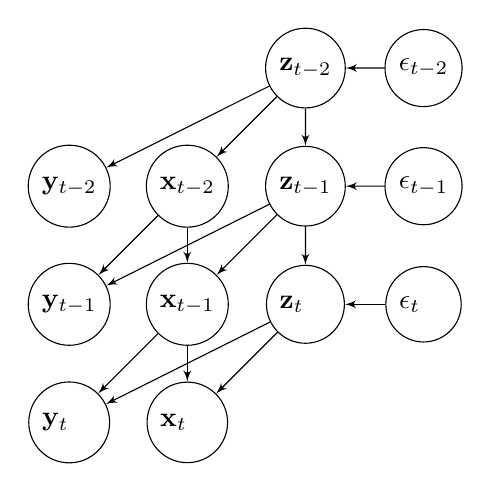
\begin{tikzpicture}[scale=1.5]
    \tikzset{
      vertex/.style={circle,draw, minimum size=2em},
      edge/.style={->,> = latex'}
    }
    % vertices
    \node[vertex] (zt) at (1 ,0) {$\mathbf{z}_{t\quad}$};
    \node[vertex] (zt1) at (1 , 1) {$\mathbf{z}_{t-1}$};
    \node[vertex] (zt2) at (1 , 2) {$\mathbf{z}_{t-2}$};
    \node[vertex] (xt) at (0 ,-1) {$\mathbf{x}_{t\quad}$};
    \node[vertex] (xt1) at (0 , 0) {$\mathbf{x}_{t-1}$};
    \node[vertex] (xt2) at (0 , 1) {$\mathbf{x}_{t-2}$};
    \node[vertex] (yt) at (-1,-1) {$\mathbf{y}_{t\quad}$};
    \node[vertex] (yt1) at (-1, 0) {$\mathbf{y}_{t-1}$};
    \node[vertex] (yt2) at (-1, 1) {$\mathbf{y}_{t-2}$};
    \node[vertex] (et) at (2 , 0) {$\mathbf{\epsilon}_{t\quad}$};
    \node[vertex] (et1) at (2 , 1) {$\mathbf{\epsilon}_{t-1}$};
    \node[vertex] (et2) at (2 , 2) {$\mathbf{\epsilon}_{t-2}$};

    %edges
    \draw[edge] (et) -- (zt);
    \draw[edge] (et1) -- (zt1);
    \draw[edge] (et2) -- (zt2);
    \draw[edge] (zt2) -- (zt1);
    \draw[edge] (zt1) -- (zt);
    \draw[edge] (xt2) -- (xt1);
    \draw[edge] (xt1) -- (xt);
    \draw[edge] (zt2) -- (xt2);
    \draw[edge] (zt1) -- (xt1);
    \draw[edge] (zt) -- (xt);
    \draw[edge] (zt2) -- (yt2);
    \draw[edge] (zt1) -- (yt1);
    \draw[edge] (zt) -- (yt);
    \draw[edge] (xt2) -- (yt1);
    \draw[edge] (xt1) -- (yt);
  \end{tikzpicture}
  \caption{DSGE solution expressed as a DAG}
  \label{dsge_dag}
\end{figure}

It would seem straightforward to input random samples generated from a DSGE model into the available structure learning algorithms in order to find the correct solution, given that these algorithms have well established asymptotic convergence properties. Unfortunately, despite extensive experimentation with these tools, I was unable to obtain any meaningful results in this way, as these algorithms seem to have a number of important limitations in this context. Constraint-based algorithms rely on conditional independence tests which themselves involve computing the correlation between residuals. In the context of simulated data these residuals may be very small or effectively zero when conditioning on the true parents of a node. In this case the computation of partial correlations may be unstable and lead to spurious results. Furthermore, these results are only asymptotic and it seems that finite-sample bias may be important in economic applications, where sample sizes are small. Particularly problematic is that structure learning algorithms consider all possible DAGs given observed variables as potential candidates, whereas in this context we assume that the solution takes on a particular form, as in equations (\ref{ss_solution:x}) - (\ref{ss_solution:z}).

As a result of these limitations, a more effective approach in this context is to design a bespoke algorithm that takes into account the relatively stringent assumptions that can be made about DSGE solutions. For the reasons outlined in section \ref{dag_estimation} this will be a hybrid algorithm. Therefore, before introducing the algorithm we will define relevant constraint and score tests in turn.

\subsection{Constraint Tests} \label{constrainttests}

\subsubsection{Independence Relationships}

Assuming the DAG in Figure \ref{dsge_dag} is faithful to the DGP specified by equations (\ref{ss_solution:x}) - (\ref{ss_solution:z}) the parental Markov condtion implies the following four independence relationships among the time $t$ and $t-1$ variables:

\begin{align}
  x_t \indep x^{\prime}_{t} \,||\,& [\mathbf{x}_{t-1},\mathbf{z}_t] \text{ for all } x_t \neq x^{\prime}_{t} \in [\mathbf{x}_t, \mathbf{y}_t] \label{constraint_test:1} \\
  x_{t-1} \indep z_{t} \,||\,& \mathbf{z}_{t-1} \text{ for all } x_{t-1} \in \mathbf{x}_{t-1} \text{ and } z_{t} \in \mathbf{z}_t \label{constraint_test:3} \\
  x_t \indep z_{t-1} \,||\,& [\mathbf{x}_{t-1}, \mathbf{z}_t] \text{ for all } x_t \in [\mathbf{x}_t, \mathbf{y}_t] \text{ and } z_{t-1} \in \mathbf{z}_{t-1} \label{constraint_test:2} \\
  z_t \indep z^{\prime}_{t} || \mathbf{z}_{t-1} & \text{ for all } z_t \not = z^{\prime}_{t} \in \mathbf{z}_t \label{constraint_test:4}
\end{align}

The first condition (\ref{constraint_test:1}) is the statement that the model's time $t$ endogenous variables are explained entirely by and are therefore unconfounded conditional on $\mathbf{x}_{t-1}$ and $\mathbf{z}_t$ (the time $t$ states). In DAG parlance, a time $t$ endogenous variable is \textit{d-separated} from and therefore independent of any other time $t$ endogenous variable by the time $t$ states. Condition (\ref{constraint_test:3}) states that the time $t$ states that every lagged endogenous state is independent of every exogenous state conditional on the lagged exogenous states. This follows from the exogeneity of $\mathbf{z}$ which implies that the only parent of $z_t$ other than the shock is $z_{t-1}$. Condition (\ref{constraint_test:2}) holds because the time $t$ states d-separate the time $t$ endogenous variables from the lagged exogenous states. If we were to consider further lags, this conditional independence would apply not only to $z_{t-1}$, but also to all $t-2$ and earlier variables because of the Markov condition. Finally, Condition (\ref{constraint_test:4}) holds that all exogenous states are mutually independent conditional on past exogenous shocks. This is a stronger condition than the other three, and depends crucially on the assumption that $\mathbf{E}$ and $\Sigma$ are diagonal.

We consider only independence relationships because in gneral all variables in the model are related to every other variable in the model in some way. Therfore, the \textit{lack} of a relationship in the form of conditional independence is more useful for identification. These constraint tests already provide a powerful selection criteria for empirical DSGE models I will call \textit{validity}:

\begin{definition}
  For a set of variables $\mathbf{w}$, a log-linearised DSGE model $M$ is \textit{valid} with respect to a distribution $f(\mathbf{w})$ if the exogenous states ($\mathbf{z}$), endogenous states ($\mathbf{x}$) and controls ($\mathbf{y}$) of $M$ as defined in equations (\ref{ss_solution:x}) - (\ref{ss_solution:z}) satisfy conditions (\ref{constraint_test:1}), (\ref{constraint_test:3}), and the minimum state variable criterion (MSV) \parencite{mccallum1999role}.
  \label{validity}
\end{definition}

It is proved in an appendix (\ref{proofs}) that under the assumption that the distribution generated by a log-linear DSGE model can be faithfully represented by some DAG $g$ there is exactly one DAG (and thus one partition of observed variables) that is valid. Constraints (\ref{constraint_test:2}) and (\ref{constraint_test:4}) are still applicable (necessary) because they are implied by the DAG, but there are not required to be sufficent for a unique solution. To be more general we could drop these assumptions as long as the shocks only directly effect the exogenous states, and the other constraints would still hold and be valid tests of the model. However, these constraints (and the associated assumptions) can nonetheless be included because they are satisfied by a wide range of DSGE models including all of those considered in the empirical portion of this paper, and more importantly conducting a larger number of tests will give more \textit{power} to reject incorrect models when using finite samples.

\subsubsection{Testing Procedure} \label{testing}

This section will discuss the implementation of an emperically viable strategy for testing conditions (\ref{constraint_test:1}) - (\ref{constraint_test:4}). In the present application, we make the assumption that observed variables are normally distributed, such that testing for conditional independence is equivalent to testing for partial non-correlation. This assumption is in general not required as it is possible to test for conditional independence non-parametrically (see \citeauthor{strobl2019approximate} (\citeyear{strobl2019approximate}) for a review of recent contributions in this vein), however, it is justified here as Gaussian assumptions are common in DSGE models and economic applications more generally, and they lend themselves to clear exoposition of other important concepts. 

Partial linear correlations can estimated by regressing the set of target variables of interest $\mathbf{x}$ on the set of conditioning variables $\mathbf{z}$ and then estimating the correlations between the resulting residuals $\mathbf{u}_x$. Therefore, one way to implement tests for conditions (\ref{constraint_test:1}) - (\ref{constraint_test:4}) would be to perform a t-test on the estimated partial linear correlation implied by each of these conditons for every model, and then reject the model if any of these t-tests reject the null hypothesis at the chosen nominal significance level (after applying a \citeauthor{bonferroni1936teoria} (\citeyear{bonferroni1936teoria}) correction). Hereafter this is referred to as the \textit{multiple testing approach}. This approach does seem to perform well on simulated data, with higher power and lower size than the second approach that I will soon introduce. However, it has a number of significant drawbacks. 

Firstly, the \citeauthor{bonferroni1936teoria} (\citeyear{bonferroni1936teoria}) correction assumes independence of each of tests, which is highly implausible in this case. Indeed, this explains why the emperical size of these tests is less than the nominal significance level. It is difficult or impossible to pin down important statistical properties (such as the size or power) of this estimator. Furthermore, there is the issue that computation of partial correlations can be unstable if residuals are very close to or equal to zero. This is precisely what is observed in applications to simulated data, where the residuals produced by the ground truth model will be zero. In general, correlation is undefined in this case, but in practice it tends to 1. This is problematic because this is exactly when we do not want to reject the null hypothesis of conditional independence. The only way around this is to detect small residuals below some tolerance threshold and pass the model through the test (do not reject the hypothesis of independence) if they are observed. Finally, the number of tests conducted can grow very large if there is a large number of observables resulting in implausibly large critical values, and growing computaional complexity.

For these reasons, I also propose the implementation of a different test provided by \citeauthor{srivastava2005some} (\citeyear{srivastava2005some}). This test is for the null hypothesis that a covaraince matrix is diagonal. In order to use this, we will combine conditions (\ref{constraint_test:1}) - (\ref{constraint_test:4}) such that they have the same conditioning set, and imply a relationship of \textit{complete independence} between tested variables. To do this, roll conditions (\ref{constraint_test:1}) and (\ref{constraint_test:2}) back 1 period \footnote{Equivalently, one could roll forwards the other two conditions, but this would require data on a lead rather than two lags.}, and add $\mathbf{x}_{t-2}$ to the conditioning sets in conditions (\ref{constraint_test:3}) and \ref{constraint_test:4}. This latter change is justified because in both cases we have already blocked every backdoor path between the variables of interest and $\mathbf{x}_{t-2}$ is not part of any frontdoor path between them, and therefore d-separation is maintained. Therefore these changes do not modify the conditional independence relationships in any meaningful way. The modified conditions are shown in (\ref{mod_constraint_test:1}) - (\ref{mod_constraint_test:4}).

\begin{align}
  x_{t-1} \indep x^{\prime}_{t-1} \,||\,& [\mathbf{x}_{t-2},\mathbf{z}_{t-1}] \text{ for all } x_{t-1} \neq x^{\prime}_{t-1} \in [\mathbf{x}_{t-1}, \mathbf{y}_{t-1}] \label{mod_constraint_test:1} \\
  x_{t-2} \indep z_{t-1} \,||\,& [\mathbf{x}_{t-2},\mathbf{z}_{t-1}] \text{ for all } x_{t-1} \in \mathbf{x}_{t-1} \text{ and } z_{t-1} \in \mathbf{z}_{t-1} \label{mod_constraint_test:3} \\
  x_{t-1} \indep z_{t-2} \,||\,& [\mathbf{x}_{t-2},\mathbf{z}_{t-1}] \text{ for all } x_{t-1} \in [\mathbf{x}_{t-1}, \mathbf{y}_{t-1}] \text{ and } z_{t-2} \in \mathbf{z}_{t-2} \label{mod_constraint_test:2} \\
  z_{t-1} \indep z^{\prime}_{t-1} || & [\mathbf{x}_{t-2},\mathbf{z}_{t-1}] \text{ for all } z_{t-1} \not = z^{\prime}_{t-1} \in \mathbf{z}_{t-1} \label{mod_constraint_test:4}
\end{align}

We now have that every condition relies on the same conditioning set. Furthermore, when combined these conditions imply that all of the variables in the vector $[\mathbf{y}_{t-1}, \mathbf{x}_{t-1}, \mathbf{z}_{t}, \mathbf{z}_{t-2}]$ are completely independent, conditional on $[\mathbf{x}_{t-2}, \mathbf{z}_{t-1}]$. $\mathbf{z}_{t-2}$ can be optionally excluded from this vector as it is associated with test (\ref{constraint_test:2}), which is not required for a unique \textit{valid} model. On the other hand we will have to impose (\ref{constraint_test:4}), which is also not required in order to implement this test. This is not the case for the multiple testing strategy. To test whether a model is valid emperically, we then estimate the covariance matrix $S$ of the $n$ x $m$ vector $[\mathbf{y}_{t-1}, \mathbf{x}_{t-1}, \mathbf{z}_{t}]$, and perform a z-test at some nominal significance level $\alpha$ on the test statisic $T_3$ from \citeauthor{srivastava2005some} (\citeyear{srivastava2005some}), which is asymptotically normally distributed. This test statisic is defined in (\ref{t3}) - (\ref{a40}):

\begin{align}
  \hat{T}_3 = \left(\frac{n}2{}\right)\frac{(\hat{\gamma}_3-1)}{\left(1-\left(\frac{1}{p}\right)\left(\frac{\hat{a}_{40}}{\hat{a}^2_{20}}\right)\right)^\frac{1}{2}} \label{t3} \\
  \hat{\gamma}_3 = \frac{n}{n-1}\frac{tr(S^2) - \frac{1}{n}(tr(S))^2}{\sum_{i=1}^ms^2_{ii}} \\
  \hat{a}_{20} = \frac{n}{p(n+2)}\sum_{i=1}^ms^2_{ii} \\
  \hat{a}_{40} = \frac{1}{p}\sum_{i=1}^ms^4_{ii} \label{a40}
\end{align}

Where $s_{ij}$ is the $(i,j)$ element of $S$. Note that the denominator in $\hat{T}_3$, $\left(1-\left(\frac{1}{p}\right)\left(\frac{\hat{a}_{40}}{\hat{a}^2_{20}}\right)\right)$ can be negative, and thus, the test statistic undefined. In order to alliviate this I take the same approach as in \citeauthor{wang2013necessary} (\citeyear{wang2013necessary}) and replace this term with $1-\sum_{i=1}^ms^4_{ii}/\left(\sum_{i=1}^ms^2_{ii}\right)^2$ when it is negative.

This strategy solves a number of the drawbacks of the first approach, however, as we will see in Section \ref{results}, despite being faster computationally, it unfortunately does not seem to be as accurate in simulations on more complex data sets as the multiple testing strategy. Since this approach utilises estimated covariance rather than correlations it avoids unstable computation around the true model, where residauals are very close to zero. Therefore, we are able to test all models without making exceptions for special cases. Furthermore, it is much simpler to describe the properties of this test. Asymptotically, it will have exactly $\alpha$ type I error rate. Estimates of the power of this test against numerous alternatives can be found in \citeauthor{wang2013necessary} (\citeyear{wang2013necessary}). Estimates of the emperical size and power of this test over a range of scenarios are also provided in Appendix \ref{testing_validation}. Finally, this test results in exactly one test being perfomed regardless of the complexity of the data or model under consideration. While it is true that the test is somewhat more computationally intensive for larger covariance matrices, it scales much better than the other approach. 

\subsection{Score Tests} \label{scoretests}

In finite samples it is not uncommon to encounter cases where more than one model is valid. These models will generally be very similar to the ground truth, and represent a small minority of all considered models. Therefore, one possible approach is to find the set of emperically valid models and then select from these manually. However, in order to achieve a maximally agnostic algorithmic approach that still yields a unique solution we will instead implement a score function. Essentially, this will sort the models which are deemed to be valid by their predictive accuracy or likelihood in order to choose a unique winning model. In principle, one could evaluate models solely on their score, however, for the reasons outlined in Section \ref{dag_estimation}, my prefered approach is to use this only in a secondary role. For comparision simulation results for pure score-based estimation will be  considered in Section \ref{results}.

The most basic score function for Gaussian Bayesian networks is the log-likelihood function. The Markov compatibility condition (Definition \ref{markovcompatibility}) DAG admits factorisation of the joint probability distribution into the product of the distribution of each variable conditional on its parents:

\begin{equation}
  f(\mathbf{w};\theta) = \prod_{i=1}^{k} f(w_i | pa_i;\theta)
\end{equation}

Therefore, the log-likelihood can be calculated as:

\begin{equation}
  \mathcal{L}(\mathbf{w},\theta) = \sum_{i=1}^{k} ln(f(w_i | pa_i;\theta))
\end{equation}

Now consider the assumptions in the current context. $\mathbf{w_i}$ is partitioned into $\mathbf{z}$, $\mathbf{x}$, and, $\mathbf{y}$. We assume that the conditional probabilities are linear functions and follow a mean-zero normal distribution, so the only parameter is the variance-covariance matrix $\tilde{\Sigma}$. Furthermore, the model predicts time $t$ values \textit{given} time $t-1$ values so we do not need to consider the distribution of lags. Therfore,

\begin{align}
  \mathcal{L}(\mathbf{w}; \mathbf{A}, \mathbf{B}, \mathbf{C}, \mathbf{D}, \mathbf{E}, \mathbf{\sigma}^2) =& \sum_{z_{i,t} \in \mathbf{z}_t} \bigg{(} \sum_{t=1}^{T} ln(\phi(z_{i,t} | z_{i,t-1} | \mathbf{E}, \tilde{\Sigma}_z)) \bigg{)} \nonumber\\
  +& \sum_{y_{i,t} \in [\mathbf{y}_t,\mathbf{x}_t]} \bigg{(} \sum_{t=1}^{T} ln(\phi(y_{i,t} | [\mathbf{x}_{t-1}, \mathbf{z}_{t}] | \mathbf{A}, \mathbf{B}, \mathbf{C}, \mathbf{D}, \tilde{\Sigma}_y)) \bigg{)} \\
  =& \sum_{y_{i,t} \in \mathbf{y}_t} \bigg{(} \sum_{t=1}^{T} ln(\phi(\mathbf{a}_i \mathbf{x}_{t-1} + \mathbf{b}_i \mathbf{z}_t | \mathbf{a}_i, \mathbf{b}_i, \sigma_i^2)) \bigg{)} + \nonumber\\
  & \sum_{x_{i,t} \in \mathbf{x}_t} \bigg{(} \sum_{t=1}^{T} ln(\phi(\mathbf{c}_i \mathbf{x}_{t-1} + \mathbf{d}_i \mathbf{z}_t | \mathbf{c}_i, \mathbf{d}_i, \sigma_i^2)) \bigg{)} \nonumber\\
  & \sum_{z_{i,t} \in \mathbf{z}_t} \bigg{(} \sum_{t=1}^{T} ln(\phi(\mathbf{e}_i z_{i,t-1}  | \mathbf{e}_i, \sigma_i^2)) \bigg{)}
\end{align}

Where $\mathbf{x_i}$ is the $i_{th}$ row of $\mathbf{X_i}$, $\sigma_i^2$ are the diagonal elements of $\tilde{\Sigma}$, and $\phi$ is the probability density function of the normal distribution. Notice that we can calculate the variances separately in each linear projection because the parental Markvov condition implies that they are independent. Finally, we can substitute in for the maximum likelihood estimate of $\sigma_i^2$ for each regression and the functional form of $\phi$ to arrive at an expression for the log-likelihood function:

\begin{align}
  \mathcal{L(\mathbf{w})} =& -\frac{T}{2} \bigg{(} 
  k (1 + ln(2\pi)) 
  + \sum_{i=1}^{k} ln(\hat{\sigma}_{i}^2)
  \bigg{)} \\
  \hat{\sigma}_{i}^2 =& \frac{1}{T} \sum_{t=1}^{T} (w_{i,t} - \hat{w}_{i,t})^2
\end{align}

Where $\hat{w}_{i,t}$ is are of predicted values of some $w_i$ in $\mathbf{w}$ implied by estimates of equations (\ref{ss_solution:x}) - (\ref{ss_solution:z}) using the maximum-likelihood estimates of the coefficient matrices.

Since maximising the log-likelihood does not penalise complexity, it often favours models with many more edges than exist in the ground truth. In other words, maximising log-likelihood over a space of candidate DAGs may lead to \textit{overfitting}. The most common response to this is to use a penalised score function such as the Akaike Information Criterion (AIC) \parencite{akaike1974new} and the Bayesian Information Criterion (BIC) \parencite{schwarz1978estimating}. Given that we are already applying stringent conditional independence criteria, it may seem that this bias towards complexity is irrelevant. However given the minimal number of states, it is still possible to reallocate between exogenous and endogenous states. In this context the bias towards complexity means a we are likely to choose more exogenous states than truly exist, since these involve the estimation of more parameters than endogenous states, and since they enter at time $t$ instead of time $t-1$ they likely contain more relevant information about time $t$ endogenous variables. In practice, penalised score functions are very unlikely to overturn this complexity bias. So instead of using these, I will simply take preference for models with more endogenous states first, and then only after this maximise the likelihood function. The justification for this choice is that in macroeconomics we generallly believe that all observables are interrelated in some way, and therefore, the exogeneity assumptions implied by exogenous states are quite strong and it is thus preferable to minimise them. 

\subsection{Algorithm} \label{algo}

Having defined a number of tests for an optimal and \textit{valid} model, we now turn our attention to developing an algorithm which will apply these tests in order to choose one from the space of all possible state-space models.

\begin{minipage}{\linewidth}
  \begin{algorithm}[H]
    \SetAlgoLined
    \DontPrintSemicolon
    
    % python like syntax
    \SetStartEndCondition{ }{}{}%
    \SetKwProg{Fn}{def}{\string:}{}
    \SetKwFunction{Range}{range}%%
    \SetKw{KwTo}{in}\SetKwFor{For}{for}{\string:}{}%
    \SetKwIF{If}{ElseIf}{Else}{if}{:}{elif}{else:}{}%
    \SetKwFor{While}{while}{:}{fintq}%
    \AlgoDontDisplayBlockMarkers
    \SetAlgoNoEnd
    %\SetAlgoNoLine

    \SetKwData{Continue}{$continue$}
    \SetKwData{Nstates}{$n\_states$}
    \SetKwData{Maxstates}{$max\_states$}
    \SetKwData{Allvalidstates}{$all\_valid\_states$}
    \SetKwData{Siglevel}{$sig\_level$}
    \SetKwData{Potentialstates}{$potential\_states$}
    \SetKwData{Allpotentialstates}{$all\_potential\_states$}
    \SetKwData{Potentialstate}{$potential\_state$}
    \SetKwData{Constrainttests}{$constraint\_tests$}
    \SetKwData{Constrainttest}{$constraint\_test$}
    \SetKwData{Scoretests}{$score\_tests$}
    \SetKwData{Scoretest}{$score\_test$}
    \SetKwData{Nendo}{$\#endogenous\_states$}
    \SetKwData{States}{$states$}
    \SetKwData{True}{$true$}
    \SetKwData{False}{$false$}
    \SetKwFunction{Getpotentialstates}{$get\_potential\_states$}
    \SetKwData{Getconstrainttests}{$get\_constraint\_tests$}
    \SetKwData{Getscoretests}{$get\_score\_tests$}
    \KwIn{$alpha$: significance level}
    \KwIn{$test$: testing strategy is either 'multiple' or 'srivastava'}
    \KwOut{$all\_valid\_states$: A set of minimal sets of exogenous and endogenous states whose implied conditional independences are valid relative to the observed data}
    \Begin{
      \Continue $=$ \True\;
      \Nstates $= 0$\;
      \Maxstates $= \#observables - 2$\;
      \Allvalidstates $= list()$ \;
      \While{\Continue $and$ \Nstates $<=$ \Maxstates} {
        \Allpotentialstates $=$ \Getpotentialstates{\Nstates}\;
        \For{\Potentialstates $\in$ \Allpotentialstates}{
          \Constrainttests $=$ \Getconstrainttests{\Potentialstates}\;
          \Scoretests $=$ \Getscoretests{\Potentialstates}\;
          \If{$test$ $=$ $multiple$}{
            \Siglevel $=$ $\frac{alpha}{length(constraint\_tests)}$\;
          } \Else {
            \Siglevel $=$ $alpha$
          }
          \If{$every$ \Constrainttest $.p\_value >$ \Siglevel $for$ \Constrainttest $\in$ \Constrainttests}{
            $append$ \Potentialstates $to$ \Allvalidstates\;
            \Continue $=$ \False\;
          }
        }
      }
      $sort$ $ascending$ \Allvalidstates $by$ \Nendo, \Scoretests\;
      $return$ \Allvalidstates
  }
    \caption{Brute force hybrid state-space estimation algorithm}
    \label{constraint_algo}
  \end{algorithm}
\end{minipage} \\

The algorithm is very simple and is designed to reflect a few key model selection heuristics. As previously discussed, The algorithm assumes that the constraint validity is more important than score maximisation. The scores of models that are not valid relative to the constraints are irrelevant because these models are thrown out. The justification for this heuristic is outlined int \ref{dag_estimation}. Essentially, unlike score functions, constraints directly encode information about a relevant sense of causality.

The algorithm embodies the MSV criterion as it stops once one valid model is found. This is primarily because only models satisfying the MSV criterion are \textit{valid}, however, there are a number of other justifications. Firstly, this can be seen as the application of \textit{Occam's Razor} to state-space models, wherein state variables have more complex dynamics than controls. Consider equations (\ref{ss_solution:x}) - (\ref{ss_solution:z}). Exogenous states are involved in all three equations, endogenous states two, and controls only one. Another way to see this is in figure \ref{dsge_dag}. Among time $t$ and $t-1$ variables, adding an exogenous state results in the addition of edges in four places and thus eight parameters (one slope parameter and one variance parameter), an endogenous state in three places, and a control in only two. Therefore, models with with fewer states, especially exogenous states are more parsimonious and are therefore preferable, all else equal. The MSV criteria also allows for a potentially very large increase in the speed of the algorithm. Without it we must consider every possible combinations of states. Since the choice of states is multinomial with three categories the complexity of this algorithm is $\mathcal{O}(3^k)$. However, if the ground truth has only $m < k$ states then we can skip $\sum_{r=m}^{k} 2^r {\binom{k}{r}}$ iterations, which is potentially many orders of magnitude if $m << k$. This algorithm is nonetheless highly inefficient, however, it is still feasible in many important cases. There are undoubtedly many performance improvements which could be made to this algorithm, but this is left as a topic for for future research.

This algorithm will consistently estimate the unique valid state-space model as $n \rightarrow \infty$ with $k \equiv |\mathbf{w}|$ fixed. The test given by \citeauthor{srivastava2005some} (\citeyear{srivastava2005some}), and indeed the multiple testing strategy has asymptotic power equal to unity. Therefore, since the algorithm systematically considers every possible model, it will reject every incorrect model in the asymptotic case. It will also reject the correct model in a proportion $\alpha$ of samples. In these cases the algorithm will yield no solution. In the rest it will yield the unique valid model. 

However, in finite samples there is unfortunately no guarantee that the algorithm will yield the correct solution. Although the test from \citeauthor{srivastava2005some} (\citeyear{srivastava2005some}) is only asymptotically normal, in practice the type I error rate remains close to the specified nominal significance level $\alpha$ for any reasonable sample size (see Appendix \ref{testing_validation}). On the other hand, the probability of type II error can be quite high in small samples, and this is very problematic. The algorithm will stop early if it finds some valid model with $m$ states. However, if this is the result of a type II error, and the correct model actually has $>m$ states, then the algorithm will terminate before it ever even considers the correct model. Potential solutions to this problem that would improve small sample performance would be to devise a test with more power, or to remove the early stopping behavior, although this would result in a greater reliance on sorting by score to differentiate between valid models, and greatly increased runtime in most applications.

\subsection{Related Modelling Techniques}

Having discussed how DSGE models and macroeconomic data more generally can be represented as DAGs this section will discuss how this approach relates to other econometric approaches which are common in the analysis of macroeconomic timeseries. It is possible to draw comparisions with both Structural Vector Autoregression (SVAR) and Autoregessive Distributed Lag (ADL) models, so these will be discussed in turn.

One of the most common and simplest econometric models for this type of data is the vector autoregression (VAR), which was introduced by \citeauthor{sims1980macroeconomics} (\citeyear{sims1980macroeconomics}). This method involves regressing a vector of outcomes $y_t$ on a matrix containing $k$ lags of $y$ in the form $y_t = [y_{t-1}, ..., y_{t-k}] \beta + \epsilon_t $. The primary concern with and limitation of this approach is that the estimated covariance matrix $\epsilon_t$ is unrestricted, so the shocks contained within it are not mutually independent. Therefore, this model can not be used to estimate the effect of a truely exogenous shock on the dynamics of observed variables. In order to address this issue the model is transformed and an assumed causal ordering is imposed in the form of a Cholesky decomposition \parencite{sims1980macroeconomics}, which has the effect of making the errors of the estimated, transformed model mutally uncorrelated or \textit{structural}. Therefore, such models are known as SVARs. As noted by \citeauthor{demiralp2003searching} (\citeyear{demiralp2003searching}), in this context there is an equivallence between SVAR models and DAGs. This is because root nodes are assumed to be mutually uncorrelated, and as a result, any shocks to these will have a structural interpretation.

However, one key difference between a DAG in this context and a SVAR model is that the DAG allows for some variables to depend on contemporanious values of other variables. In particular, the endogenous states and controls depend contemporaniously on the exogenous states. In this sense the DAG is similar to an Autoregressive Distributed Lag (ADL) model. When implementing an ADL model it is necessary for the researcher to choose which contemporanious variables to include as regressors, implicitly assuming that this regressors are at least weakly exogenous relative to the outcomes of interest. 

The primary advantage of DAGs is the relatively weak assumptions they require. Both the SVAR and ADL models require the researcher to specify assumptions about the relative exogeneity of observable variables. These assumptions are themselves either derived from a similarly assumption-heavy model such as a DSGE model, or are entirely \textit{ad hoc}. There has been a long tradition within the field of economics including seminal papers by \citeauthor{lucas1976econometric} (\citeyear{lucas1976econometric}), \citeauthor{sims1980macroeconomics} (\citeyear{sims1980macroeconomics}), and \citeauthor{jorda2005estimation}, (\citeyear{jorda2005estimation}) criticising this type of model building. DAGs consitute a powerful new tool to choose the specification of these types of models in an agnostic and data-driven way.

\subsection{IRFs}

One very common way of evaluating DSGE models is to compare the Impulse Response Functions (IRFs) they imply and to compare those with the IRFs of reduced form models such as VAR models \parencite[p.83]{ramey2016handbook}. This is also possible when directly estimating state-space models, and the results of this will be considered in the empirical section of this paper. This is done to demonstrate that the state-space model that is estimated matches the reduced form of the original simulation. IRFs are calculated, starting with a vector of initial values (shocks), by iteratively using the estimated matrices $\hat{\mathbf{A}}$ = $\hat{\mathbf{E}}$ to calculate current time step values using past values. Note that this can be done for either exogenous or endogenous states, but not for controls, as changes to these are by construction not propagated through to future time steps.

\section{Data} \label{data}

In order to demonstrate the capability of the DAG methodology empirically I will work with both simulated and real macroeconomic data. Using simulated data has a number of key advantages. Firstly, since the model that generates the data is known it is possible to evaluate whether structure learning has succeeded in identifying the ground-truth DAG. Secondly, in this context it is possible to ensure to the greatest possible extent that the underlying assumptions of the structure learning algorithms, including linearity and normality are satisfied. Finally, since these models are central to modern macroeconomics it provides a controlled testing environment which is also arguably highly relevant to real data. On the other hand, using real data is an opportunity to demonstrate that DAGs are also a powerful heuristic tool that can be implemented outside of a rigorously controlled environment. Furthermore, if these results are to be believed it will allo for inferences pertaining to a number of important debates in the DSGE literature. The remainder of this section will discuss the various sources and general properties of the data used in this paper.

\subsection{Simulations}

In order to collect simulated data I consulted a github repository containing Dynare code to replicate well known macroeconomic models \parencite{pfeifer2020}. In particular, I chose to model the baseline RBC model as a simple case and a New Keynesian model from \citeauthor{gali2015monetary} (\citeyear{gali2015monetary}) for a more difficult and complex modelling challenge. I modified the simulation code slightly such that simulations would output a file containing $n$ observations of $i.i.d.$ draws of the exogenous shocks, and the associated observed values of the other variables in the model. This file was then used as the input for the structure learning algorithm.

\subsubsection{Baseline RBC}

\begin{table}
  \centering
  \begin{tabular}{|l|l|l|}
    \hline
    Symbol & Name & Type \\
    \hline
    $g$ & government spending & exogenous state \\
    $z$ & technology & exogenous state \\
    $k$ & capital & endogenous state \\
    $w$ & wage rate & control \\
    $r$ & return to capital & control \\
    $y$ & output & control \\
    $c$ & consumption & control \\
    $l$ & hours worked & control \\
    $i$ & investment & control \\ \cline{2-2}
    \hline
  \end{tabular}
  \caption{Description of variables for the baseline RBC model.}
  \label{rbc_data}
\end{table}

The baseline RBC model includes 11 variables which are summarised by Table \ref{rbc_data}. This model contains two exogenous state variables: technology ($z$) and government spending ($g$), and one endogenous state: capital ($k$). There are two shocks in the model: $eps_z$ that affects only technology directly and $eps_g$ that affects only government spending directly. As explained in section \ref{dsge} these shocks are dropped from the data. The shocks are Gaussian and orthogonal, and furthermore the model is taken as a first-order approximation. Therefore, all of the necessary assumptions are satisfied

This model was chosen as it is one of the simplest DSGE models and provides a good baseline to demonstrate the effectiveness of this methodology. In particular, the default calibration of this model which was used has autoregressive coefficients on the exogenous technology and government spending processes that are very close to one, and as a result there is a high degree of persistence in all variables in the model. this model will test the algorithms performance when the assumption of stationarity is challenged.

\subsubsection{Baseline New Keynsian}

\begin{table}
  \centering
  \begin{tabular}{|l|l|l|}
    \hline
    Symbol & Name & Type \\
    \hline
    $nu$ & policy rate & exogenous state \\
    $a$ & technology & exogenous state \\
    $z$ & preferences & exogenous state \\
    $p$ & price level & endogenous state \\
    $y$ & output & control \\
    $i$ & nominal interest & control \\
    $pi$ & inflation & control \\
    $y\_gap$ & output gap & control \\
    $r\_nat$ & natural interest rate & control \\
    $r\_real$ & real interest rate & control \\
    $n$ & hours worked & control \\
    $m\_real$ & real money balances & control \\
    $m\_nominal$ & nominal money balances & control \\
    $w$ & nominal wages & control \\ 
    $c$ & consumption & control \\
    $w\_real$ & real wages & control \\
    $mu$ & mark-up & control \\ \cline{2-2}
    \hline
  \end{tabular}
  \caption{Description of variables for the baseline New Keynesian model.}
  \label{nk_data}
\end{table}

New Keynesian models are extremely popular in modern macroeconomics and are also considerably more complex than the baseline RBC. Therefore this serves as a worthy test for this methodology. In particular, I use a model from \citeauthor{gali2015monetary} (\citeyear{gali2015monetary}) as provided by \citeauthor{pfeifer2020} (\citeyear{pfeifer2020}). The variables in this model are summarised in Table \ref{nk_data}  \footnote{Some control variables which were just linear functions of another variable were dropped, for example, annualised rates.}. This model has a total of four state variables: three exogenous states (policy rate, technology and, preferences) for which there is one $i.i.d.$ and Gaussian shock each, and one endogenous (price level) state.

\subsection{US Data}

\begin{table}
  \centering
  \begin{tabular}{|l|l|}
    \hline
    Symbol & Name \\
    \hline
    $pi$ & CPI Inflation \\
    $rm$ & Federal Funds Rate (Return to Money) \\
    $g$ & (Real) Government Expenditure \\
    $y$ & (Real) GDP \\
    $i$ & (Real) Private Investment \\
    $w$ & Median (Real) Wage \\
    $rk$ & Return to Capital \tablefootnote{Estimated as average return to the NASDAQ in each quarter.} \\
    $z$ & Total Factor Productivity \\
    $u$ & Unemployment \\
    $l$ & Total Workforce \\
    $c$ & (Real) Personal Consumption \\\cline{2-2}
    \hline
  \end{tabular}
  \caption{Description of Variables for US Data}
  \label{tab3}
\end{table}

To provide an example of real macroeconomic time-series, quarterly data from the US during the period 1985-2005 were collected from FRED (\citeyear{fred2020data}) for 15 variables outlined in Table \ref{tab3}. All of the variables were detrended and demeaned by taking the residuals of an estimated first order autoregression. Total factor productivity and capital stock were provided on an annual basis and were therefore interpolated quadratically. Full details of data preprocessing are available in the project repository \parencite{hall2020git}.

Since we assume a log-linear DSGE solution we by implication assume that the data is generated from a stable distribution with no structural breaks. This particular data set was chosen because it seems likely to satisfy these assumptions. In general, structural breaks are important to model correctly, however, at present incorporating these is left as an avenue for future research.

\section{Results} \label{results}

In this section many of the properties of the proposed algorithm will be thoroughly investigated. Using simulated data allows for the possibility of many experiments to test these properties in a controlled environment. In particular, for the models under consideration two tests will be considered. To demonstrate asymptotic consistency, results from the algorithm for a very large number of samples (100,000) will be provided. To demonstrate the finite sample properties, results from a large number of runs of the algorithm (1000) with a relatively small and realistic sample size (100) will be provided and discussed.

\subsection{Baseline RBC}

Using either testing strategy from Section \ref{testing} on the entire sample of 100,000 observations for the RBC model the algorithm successfully identifies the correct states, which are exogenous states $z$ and $g$, and endogenous state $k$. No other (incorrect) models are valid. This is emperical validation of the asymptotic properties of the algorithm and tests. Figure \ref{rbc_irfs} shows the impulse responses to a technology shock generated by the original simulation and the estimated model. There are almost identical, as they should be. This is a simple validation that the state-space model is equivalent to the true reduced form and that we have recovered the correct parameters using observational maximum likelihood.

\begin{figure}
  \centering
  \begin{subfigure}{0.8\textwidth}
    \centering
    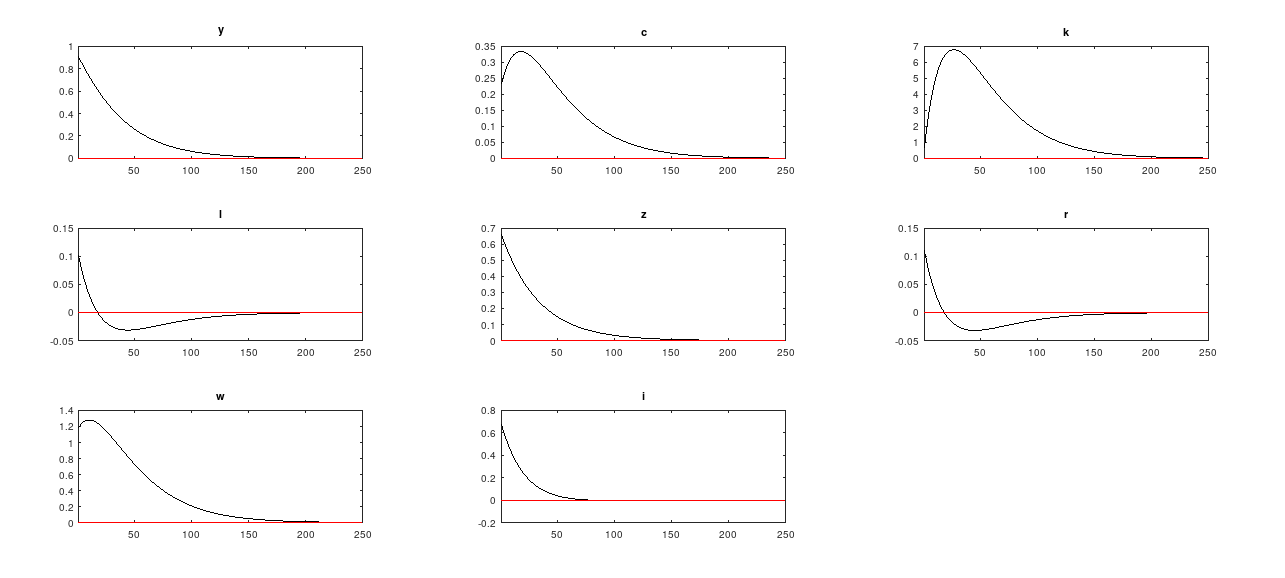
\includegraphics[width=\linewidth]{images/rbc_sim_irf.png} 
    \caption{Original Simulation}
    \label{rbc_simirf}
  \end{subfigure}
  %
  \begin{subfigure}{0.8\textwidth}
    \centering  
    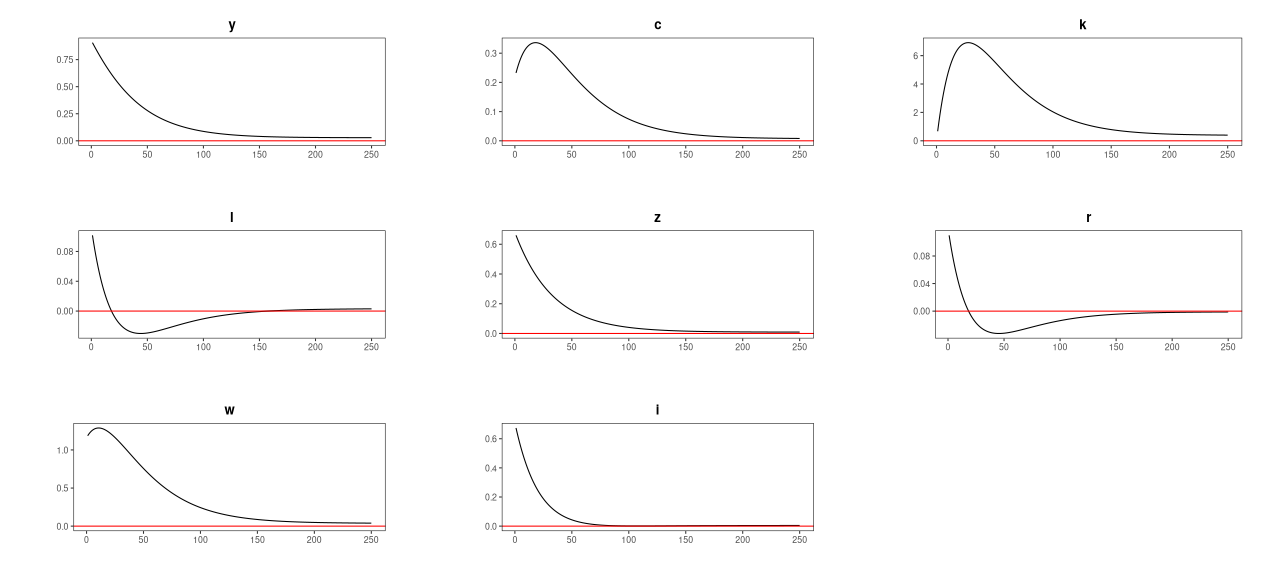
\includegraphics[width=\linewidth]{images/rbc_true_dag_irfs.png}
    \caption{Ground Truth DAG / Estimated DAG}
    \label{rbc_gtirf}
  \end{subfigure}

  \caption{IRFs to a one standard deviation technology shock generated by the original simulation and estimated model.}
  \label{rbc_irfs}
\end{figure} 

\begin{table}
  \centering
  \begin{tabular}{|c|c|c|l|l|}
    \bfseries Index & \bfseries Exogenous States & \bfseries Endogenous States & \bfseries Wins & \bfseries Valid
    \csvreader[head to column names]{./files/rbc_wins_srivastava.csv}{}
    {\\\index & \exostates & \endostates & \wins & \valid}
  \end{tabular}
  \caption{Small-sample (n=100) simulation structure learning results for RBC model using the \citeauthor{srivastava2005some} (\citeyear{srivastava2005some}) test.}
  \label{rbcwins_sr}
\end{table}

\begin{table}
  \centering
  \begin{tabular}{|c|c|c|l|l|}
    \bfseries Index & \bfseries Exogenous States & \bfseries Endogenous States & \bfseries Wins & \bfseries Valid
    \csvreader[head to column names]{./files/rbc_wins_multiple.csv}{}
    {\\\index & \exostates & \endostates & \wins & \valid}
  \end{tabular}
  \caption{Small-sample (n=100) simulation structure learning results for RBC model using pairwise correlation tests and a \citeauthor{bonferroni1936teoria} (\citeyear{bonferroni1936teoria}) correction.}
  \label{rbcwins_mu}
\end{table}

Table \ref{rbcwins_sr} shows the small sample results for the algorithm using the test based on \citeauthor{srivastava2005some} (\citeyear{srivastava2005some}), and Table \ref{rbcwins_mu} likewise for the pairwise correlation testing strategy. We will now discuss each of these results in turn.

The results in Table \ref{rbcwins_sr} are promising for a number of reasons. The headline result is that the ground-truth model (with exogenous states $g$ and $z$ and endogenous state $k$) is selcted as the optimal model by the algorithm ("wins") in nearly 95\% of iterations, and in every iteration where it is valid. The latter observation suggests that sorting by number of endogenous states and the likelihood function is having the intended effect. Also note that the emperical size of the test is quite close to the expected 5\% nominal significance level, as the correct model was rejected 56 times out of 1000 iterations ($\sim 5.6\%$). We can see that out of the 834 models that are considered in each iteration, that is the models with less than or equal to three state variables, only 17 ($\sim 2\%$) are ever valid, and of those only four (including the true model) are ever selected as the optimal model by the algorithm. Therefore, this testing strategy seems to have strong power to reject incorrect models in this application. 

Table \ref{rbcwins_mu} mirrors the previous results in many ways, however, there are some key differences. The correct model is only rejected in 3 out of the 1000 iterations, so the empirical size is far below the 5\% nominal significance level. This confirms suspicions that these pairwise correlation tests are not independent. However, this low type I error rate does not seem to have come at the cost of power, at least in comparison to the other testing strategy. Here only 8 out of the 834 models considered were ever valid, so this testing strategy actually seems to have higher power. Nonetheless, the true model does win less often using this approach (only 888 times as compared with 944), primarily because the model with exogenous states $c$ and $l$ wins 109 times (every time it is valid). This particular model was rejected in every iteration of the \citeauthor{srivastava2005some} (\citeyear{srivastava2005some}) test, despite its overall lower power. It seems likely that this model scores so highly because these $c$ and $l$ have very high autoregressive coefficients ($0.994$ and $0.972$ respectively), and as a result they get a high likelihood score when treated as exogenous states compared with $g$ and $z$, while themselves being highly correlated with $g$ and $z$ such that the prediction while treating $g$ and $z$ as controls also gets a relatively high likelihood score. The conclusion here is that the algorithm may run into difficulties in small samples if there is a high degree of multicollinearity or autocorrelation amongst variables. 

\subsection{Baseline New Keynesian}

We now turn our attention to the more complex baseline New Keynesian model\footnote{Results for the Srivastava test on this data set are in the works. Currently it is not performing well and I need to determine if this is due to a fundatmental limitation or simply a mistake.}. This model contains 17 observables, and is thus considerably more complex than the simulated RBC data. Table \ref{nk_full_mu} shows the results for a large sample. Only two models are valid, and the correct model with exogenous states $a$, $nu$, and, $z$ and endogenous state $p$ wins both on preference for endogenous states and on log likelihood. This once again consistutes emperical validation of asymptotic properties.

\begin{table}
  \centering
  \begin{tabular}{|c|c|c|c|}
    \bfseries Index & \bfseries Exogenous States & \bfseries Endogenous States &  \bfseries Log Likelihood
    \csvreader[head to column names]{./files/nk_full_multi.csv}{}
    {\\\index & \exostates & \endostates & \loglik}
  \end{tabular}
  \caption{Large sample (n=100,000) simulation structure learning results for New Keynesian model using pairwise correlation tests and a \citeauthor{bonferroni1936teoria} (\citeyear{bonferroni1936teoria}) correction.}
  \label{nk_full_mu}
\end{table}

\begin{table}
  \centering
  \begin{tabular}{|c|c|c|l|l|}
    \bfseries Index & \bfseries Exogenous States & \bfseries Endogenous States &  \bfseries Wins & \bfseries Valid
    \csvreader[head to column names]{./files/nk_wins_multiple.csv}{}
    {\\\index & \exostates & \endostates & \wins & \valid}
  \end{tabular}
  \caption{Small-sample (n=100) simulation structure learning results for New Keynesian model using pairwise correlation tests and a \citeauthor{bonferroni1936teoria} (\citeyear{bonferroni1936teoria}) correction. 55 models were valid in at least one iteration, but the table was truncated to include only those that won at least once.}
  \label{nkwins_mu}
\end{table}

Table \ref{nkwins_mu} shows the small sample results using the multiple testing strategy. The results are not as strong as with the RBC model, but this is to be expected given the greater number of variables and complexity of model considered with the same sample size. We find that the ground-truth model wins in approximately $75\%$ of iterations, while only be rejected once. 55 models were valid in at least one iteration, which represents approximately $0.1\%$ of models tested in each iteration. So despitie the complexity of this problem, the actual type I and type II error rates of the multiple testing strategy in this application were actually very low. It seems reasonable to conclude that the primary reason the true model did not win more often was because the score sorting did not perform as well as it did with the RBC model. This is because in any given iteration there are more models that are valid, and thus more competition.

These results show that there is are practical limitations to how well the algorithm and tests can perform. The tests are consistent as the sample size $n \rightarrow \infty$ with the number of observables $k$ fixed. If $k$ is not so small compared to the sample size then there is likely to be poor performance. This is a problem common to practically all econometric models, however, it may be particularly acute here because the number of models considered, and thus the complexity of the problem grows expontially in the number of observables.

\subsection{US Data}

\begin{table}
  \centering
  \begin{tabular}{|c|c|c|c|}
    \bfseries Index & \bfseries Exogenous States & \bfseries Endogenous States & \bfseries Log Likelihood
    \csvreader[head to column names]{./files/realresults_multiple.csv}{}
    {\\\index & \exostates & \endostates & \loglik}
  \end{tabular}
  \caption{Structure learning results for the US macroeconomic data set (1985-2005) using pairwise correlation tests and a \citeauthor{bonferroni1936teoria} (\citeyear{bonferroni1936teoria}) correction.}
  \label{real_mu}
\end{table}

Table \ref{real_mu} shows results for structure learning on the US macroeconomic data set using the multiple testing methodology. Despite the small data set of only 80 observations these tests were able to reject all but two of the 93434 models considered. Many features of this solution are consistent with what standard intuitions would imply. For example, we observe that capital and the policy rate are endogenous states. Both of these are standard features of any DSGE model, and the second one reflects the well studied \citeauthor{taylor1993discretion} (\citeyear{taylor1993discretion}) rule. Also note that TFP is exogenous, which is fairly standard outside of endogenous growth models.

If we are to believe these results, then there are numerous implications for theory, at least in the context of the data considered here. First of all, the fact that consumption is an endogenous state is evidence in favour of the hypotheses of \citeauthor{fuhrer2000habit} (\citeyear{fuhrer2000habit}) that DSGE models should take into acount habits in consumption, thus making consumption innertial. Furthermore, we observe that inflation is an endogenous state. This is evidence related to a particularly heated debate surounding wheter inflation is purely rational and forward looking \parencite{levin2004macroeconomic}, and should therefore be modelled as a control varable, or whether inflation demonstrates persistence \parencite{christiano2005nominal}, and should therefore be modelled as a state variable. Clearly then, this evidence supports the latter hypothesis. 

Perhaps more difficult to reason about is why output and unemployment enter as exogenous states. But for these too some explaination can be suggested. Exogenous states are the only variables in the model which are directly exposed to shocks. Assuming a Cobb-Douglas style production functuion, shocks to output which are orthogonal to productivity and unemployment would have to be shocks to capital. For example, a shock to variable capacity utilisation \parencite{driver2000capacity} seems to fit this description. Similarly, unemployment may be subject to orthogonal labor market or other policy shocks. The fact that these variables enter as exogenous states suggests that these shocks are the most important in explaining the dynamics of the macroeconomy.

\section{Conclusion} \label{conclusion}

This paper has introduced a series of tests and an algorithm for data-driven causal discovery of macroeconomic state-space models. These tests are asymptotically consistent, and have been shown to perform well on at least relatively simple data sets given a realistic sample size. Results derived using this strategy can be used to gain insight into prominent debates in the DSGE literature. This consitutes a concrete example of an application in which DAGs and the causal discovery toolkit more broadly can be used in emperical economics. This approach comes with a number of benefits, chief among them that it is maximally agnostic and makes no assumptions about relationships are present in the true DGP. 

Much work remains to be done however, as this study has uncovered a number of limitations. In order to model data from more general settings it will be necessary to encorporate DGPs that are non-stationary or contain structural breaks. Extentions could be made to allow for non-linear relationships or non-Gaussian shocks. Importantly, these extensions will have to be made in a way that does not significantly sacrifice power. As we have seen, the possibility of Type II error can be problematic, especially when considering complex data sets over small sample sizes. To this end new testing strategies should be developed and applied which have greater power against alternatives. 

\newpage
\printbibliography

\newpage
\appendix
\section{Proofs} \label{proofs}

\theoremstyle{definition}
\begin{theorem}
  Let $M$ be a log-linearised DSGE model that generates a distribution $f(\mathbf{w})$ over a set of variables $\mathbf{w}$, which can be partitioned into $\mathbf{z}$, $\mathbf{x}$, and $\mathbf{y}$ (exogenous states, endogenous states, and controls). Further suppose that $M$ is \textit{faithfully represented} by some DAG $g$ of the form of figure \ref{dsge_dag} according to the partitioning of $\mathbf{w}$. Then $g$ is the unique faithful DAG that satisfies (\ref{constraint_test:1}), (\ref{constraint_test:3}) and the minimum state variable criterion.
\end{theorem}
\begin{proof}
  Suppose not. Then $M$ is faithfully represented by a DAG $h$ which is different to $g$. Since $M$ is still a log-linear DSGE solution it must still have a faithful DAG representation of the general form in figure (\ref{dsge_dag}). Therefore, the difference must be that $h$ partitions one or more of the variables in $\mathbf{w}$ differently than $g$. Define the following notation: $g_x$ is the set of variables that are categorised as endogenous states in DAG  $g$ and likewise for $h$ and other categories. \\
  Continue by considering cases: \\
  Case 1: $a \in g_y \text{ and } a \in h_x$ \\
    $g$ has fewer state variables that $h$, which therefore does not satisfy the MSV criteria. Contradiction. \\
  Case 2: $a \in g_y \text{ and } a \in h_z$ \\
    (\ref{constraint_test:3}) fails because there is a direct path from $\mathbf{x}_{t-1}$ to $a$ in $g$. Contradiction. \\
  Case 3: $a \in g_x \text{ and } a \in h_y$ \\
    (\ref{constraint_test:1}) fails because $a$ is not in the conditioning set for this test in $h$ and therefore there is an unblocked backdoor path from $a$ to the other time $t$ endogenous variables in $g$. Contradiction. \\
  Case 4: $a \in g_x \text{ and } a \in h_z$ \\
    (\ref{constraint_test:3}) fails because there is a direct path from $\mathbf{x}_{t-1}$ to $a$ in $g$. Contradiction. \\
  Case 5: $a \in g_z \text{ and } a \in h_y$ \\
    (\ref{constraint_test:1}) fails because there is a direct path from $a$ to any time $t$ endogenous variable in $g$. Contradiction. \\
  Case 6: $a \in g_z \text{ and } a \in h_x$ \\
    (\ref{constraint_test:1}) fails because there is a direct path from $a$ to any time $t$ endogenous variable in $g$. Contradiction. 
\end{proof}

\section{Testing Validation} \label{testing_validation}

\begin{table}
  \centering
  \begin{tabular}{|c|c|c|c|c|c|}
    \bfseries Emperical Size & \bfseries Alpha & \bfseries Difference & \bfseries n & \bfseries m & \bfseries Repetitions
    \csvreader[head to column names]{./files/test_validation_alpha.csv}{}
    {\\\es & \a & \d & \n & \m & \k}
  \end{tabular}
  \caption{Emperical validation of significance level of \citeauthor{srivastava2005some} (\citeyear{srivastava2005some}) test.}
  \label{test_validation_alpha}
\end{table}

\begin{table}
  \centering
  \tiny
  \begin{tabular}{|c|c|c|c|c|c|}
    \bfseries Emperical Power & \bfseries Alpha & \bfseries n & \bfseries Correlation & \bfseries m & \bfseries Repetitions
    \csvreader[head to column names]{./files/test_validation_power.csv}{}
    {\\\ep & \a & \n & \c & \m & \k}
  \end{tabular}
  \caption{Emperical validation of power of \citeauthor{srivastava2005some} (\citeyear{srivastava2005some}) test against data generated from a normal distribution where the off-diagonal elements of the covariance matrix all take on the value specified by \textit{correlation}.}
  \label{test_validation_power}
\end{table}

\end{document}
